\chapter{Etat de l'art}

\section*{Introduction}%
\addcontentsline{toc}{section}{\numberline{}Introduction}%
%Ce chapitre a pour but de faire le contour des différents concepts qui seront abordés dans le projet pour avoir une idée de ce a quoi nous nous frotterons, puis on se placera dans le contexte de l’entreprise pour laquelle nous concevons le système tout en précisant les problématiques que nous aborderons. Ensuite on fera une étude de l’existant et enfin on introduira la solution que nous proposons pour les problèmes cités plus haut.
Ici nous allons essayer de comprendre les différents concepts qui seront abordés tout au long de la réalisation de ce projet. Commençant par les systèmes décisionnels ou encore l’intelligence des affaires (Business Intelligence en Anglais), ensuite nous parlerons des entrepôts de données, les ETL, les magasins de données, les cubes OLAP, les systèmes de reporting (la visualisation des données) et enfin nous terminerons en parlant de la gestion commerciale.
%\section{Revue de la littérature}


\section{Systèmes décisionnels ou « Business Intelligence »}
Afin de mieux comprendre la finalité des systèmes décisionnels, nous nous devons de les placer dans leurs contextes et rappeler ce qu’est un système d’information.

\paragraph{}
«Le système d’information est l’ensemble des méthodes et moyens de recueil de contrôle et de distribution des informations nécessaires à l’exercice de l’activité en tout point de l’organisation. Il a pour fonction de produire et de mémoriser les informations, de l’activité du système opérant (système opérationnel), puis de les mettre à disposition du système de décision (système de pilotage)» \cite{book:3}
\paragraph{}
Les différences qui existent entre le système de pilotage (système décisionnel) et le système opérationnel (système transactionnel), du point de vue fonctionnel ou des tâches à effectuer, conduit à l’apparition des « systèmes d’information décisionnels » (S.I.D.). Ces différences seront clairement illustrées un peu plus loin dans notre document.
\paragraph{}

Les origines des SID remontent au début de l’informatique et des systèmes d’information
qui ont, tous deux, connu une grande et complexe évolution liée notamment Cette évolution se poursuit à ce jour \cite{book:1}.
\paragraph{}
Différentes définitions du décisionnel « Business Intelligence B.I. » ont étés données au fil des ans. Parmi celles-ci on trouve : 

\textit{"Le Décisionnel est le processus visant à transformer les données en informations et,
par l'intermédiaire d'interrogations successives, transformer ces informations en
connaissances."} \cite{book:2}.

\subsection{Place du décisionnel dans l’entreprise}
La figure \ref{fig:decisionnelauseindusi}, extraite de \cite{book:4}, illustre parfaitement la place qui revient au décisionnel au sein d’une entreprise. Cette place, comprend plusieurs fonctions clés de l’entreprise. Les finalités décisionnelles, étant différentes selon le poste et la fonction occupée, ont pour but d’engendrer plusieurs composantes.

\begin{figure}[H]
    \centering
    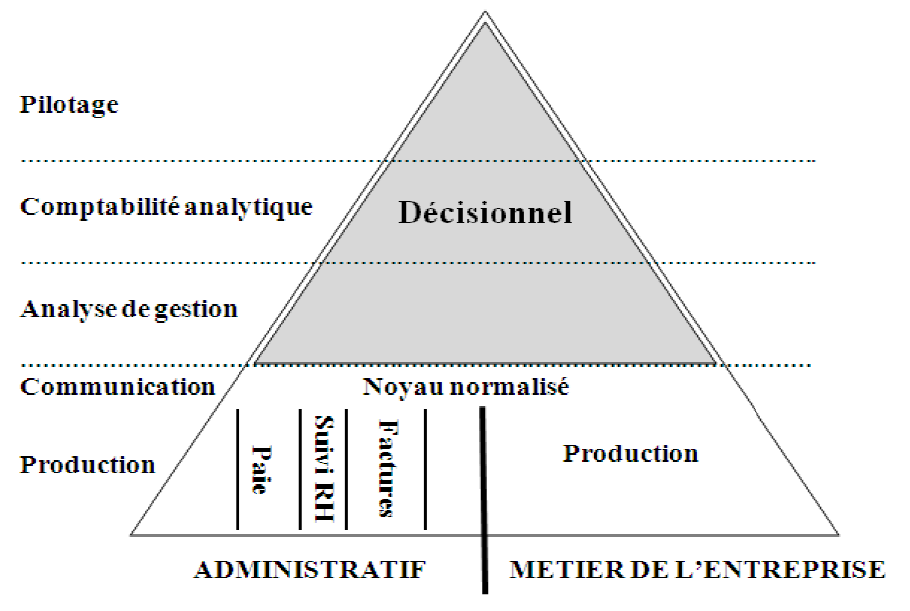
\includegraphics[width=\textwidth]{decisionnelauseindusi}
    \caption{Le décisionnel au sein du Système d’information}
    \label{fig:decisionnelauseindusi}
\end{figure}

\subsection{Différents composantes du décisionnel}
En relation étroite avec les nouvelles technologies de l’information et des télécommunications, le système décisionnel se manifeste à différents niveaux selon leurs utilités et leurs missions principales, comme illustré dans la figure \ref{fig:composantsdudecisionnel} [Goglin, 1998].

\begin{figure}[H]
    \centering
    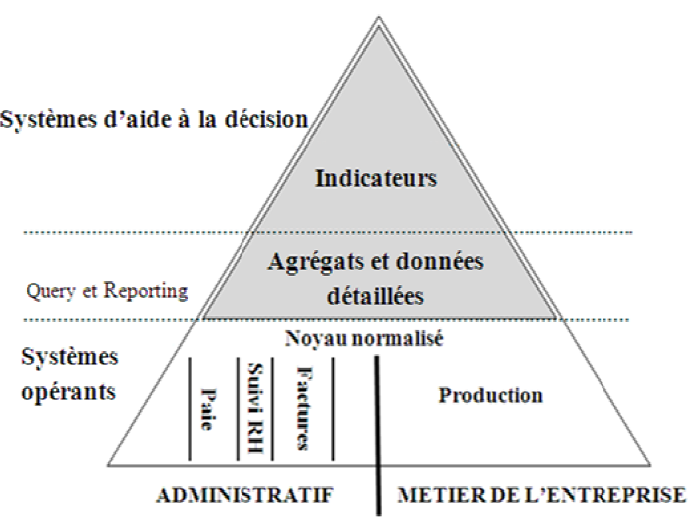
\includegraphics[width=\textwidth]{composantsdudecisionnel}
    \caption{Les différentes composantes du décisionnel}
    \label{fig:composantsdudecisionnel}
\end{figure}

\subsection{Décisionnel vs transactionnel}
Le système transactionnel permet de gérer les données en production en temps réel. Il est conçu pour l’insertion, la modification, interroger rapidement, efficacement et en sécurité les données de la base, sélectionner, ajouter, mettre à jour, supprimer des tuples et répondre à de nombreux utilisateurs simultanément.
\paragraph{}
Mais il y a des requêtes complexes et lourdes qui abîment les performances des systèmes transactionnels, et des données temporelles réparties rendent la vue historique de données difficile. Le système décisionnel gère les données agrégées, calculées selon des axes (critères d’analyse) prédéterminés à des fins d’analyse.
\paragraph{}
Le tableau \ref{tab:comparatifdecisonneltransactionnel} résume de façon non exhaustive les différences qu’il peut y avoir entre les systèmes transactionnels et les systèmes décisionnels selon les données et l’usage fait des systèmes.

\begin{table}[H]
    \centering
    \caption{Comparaison des systèmes transactionnels et les systèmes décisionnels.}
    \begin{tabular}[t]{|p{3cm}|p{6cm}|p{6cm}|} 
        \hline
        \textbf{Différence} & \textbf{Systèmes transactionnels} & \textbf{Systèmes décisionnels} \\
        \hline\hline
        \multirow{5}{5em}{Par les données} & Orienté applications & Orienté thèmes et sujets \\
        & Situation instantanée & Situation historique \\ 
        & Donnée détaillées et codées non redondantes & Informations agrégées cohérentes souvent avec redondance \\ 
        & Données changeantes constamment & Informations stables et synchronisées dans le temps \\ 
        & Pas de référentiel commun & Un référentiel unique \\ 
        \hline
        \multirow{5}{5em}{L’usage} & Assure l’activité au quotidien & Permet l’analyse et la prise de décision \\
        & Pour les opérationnels & Pour les décideurs \\ 
        & Mises à jour et requêtes simples & Lecture unique et requêtes complexes
        transparentes \\ 
        & Temps de réponse immédiats & Temps de réponse moins critiques \\ 
        & Faibles volumes à chaque transaction & Large volume manipulé \\ 
        & Conçu pour la mise à jour & Conçue pour l’extraction \\ 
        & Usage maîtrisé & Usage aléatoire \\ 
        \hline\hline
    \end{tabular}
    \label{tab:comparatifdecisonneltransactionnel}
\end{table}%


\section{Les entrepôts de données ou « Datawarehouse »}

Les entrepôts de données sont apparus en 1996, réponse au besoin de rassembler toutes les informations d’une entreprise en une base de données unique destinée aux analystes et aux gestionnaires. Celà en intègrant des informations provenant de différentes sources de données internes mais aussi externes à l’environnement de l’organisme et en offrant la possibilité de faire des analyses et des corréllations sur des agrégations crééés dynamiquement à partir de plusieurs dimentions.
\paragraph{}
Les bases de données des systèmes existants de type OLTP\footnote{Online Transaction Processing} ne sont pas appropriées comme support d’analyse, vu que leur conception ne vise pas les fonctions spécifiques réalisées dans l’entreprise. D’où la nécessité de la mise en place d’un système décisionnel qui fournit une vue globale des informations de l’entreprise et aussi un moyen stratégique de prise de décision.

\subsection{Notion de Datawarehouse}
Bill Inmon définit l’entrepôt de données dans son ouvrage "Building Data warehouse" de la façon suivante : L’entrepôt de données est une collection de données orientées sujet, intégrées, non volatiles et historiées, organisées pour support d’un processus d’aide à la décision".
\paragraph{}
Cette définition d’ED\footnote{Entrepôt de Données} a été conceptualisée en termes de caractéristiques du référentiel des données, qui seront détaillées dans les points suivants :

\begin{itemize}
    \item \textbf{Orientées sujet :} Les données de l’entrepôt sont organisées par thème (autour des sujets majeurs et des métiers de l’entreprise). L’intérêt dans cette organisation est de disposer d’un ensemble d’informations utiles sur un sujet transversal aux structures fonctionnelles et organisationnelles de l’entreprise. \cite{book:5}
    \item \textbf{Intégrées :} Les données dans l’entrepôt proviennent de différentes sources éventuellement hétérogènes. L’intégration est un processus qui consiste à résoudre les problèmes d’hétérogénéité, où les données contenues dans ED sont divisées en grandes subdivisions appelées domaine. \cite{book:6}
    \item \textbf{Non volatiles :} Les données stockées au sien de l’entrepôt sont permanentes et ne peuvent être modifiées, et le rafraîchissement de l’entrepôt de données, consiste seulement à ajouter de nouvelles données sans modifier ou perdre celle qui existent. Ceci pour conserver la traçabilité des informations et des décisions prises. \cite{book:6}
    
    \begin{figure}[H]
        \centering
        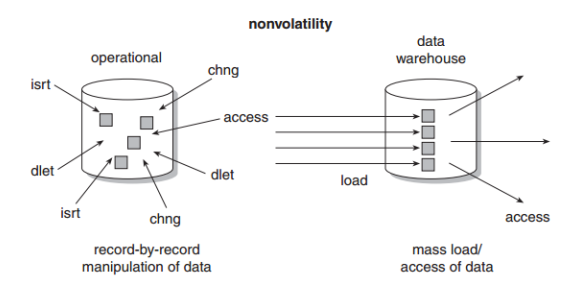
\includegraphics{nonvolatilitedonnees}
        \caption{Non volatilité des données de l’ED.}
        \label{fig:composantsdudecisionnel}
    \end{figure}

    La figure \ref{fig:composantsdudecisionnel} extrait de l'ouvrage de William Ilmon 'Building the Datawarehouse' \cite{book:7} démontre la non volatilité des données dans les entrepôt de données.

    \item \textbf{Historisées :} Pour suivre dans le temps l’évolution des différentes valeurs des indicateurs à analyser, l’historisation est nécessaire. Un référentiel de temps est associé aux données, afin de permettre l’identification dans la durée de valeurs précise. \cite{book:5}
\end{itemize}


\subsection{Historique des Datawarehouses}
L’origine des ED revient à 1960, ou l’entreprise General Mills et l’Université Dartmouth, dans un projet conjoint, créent les termes "faits" et "dimensions".Les dates marquantes de l’histoire des entrepôts de données sont : \cite{book:8}
\begin{itemize}
    \item En \textbf{1983}, Teradata introduit dans son SGBD un système purement décisionnel.
    \item En \textbf{1988}, Le terme DataWarehouse est utilisé pour la premiere fois dans l’article "An architecture for business and information systems" publier par Barry Devlin et Paul Murphy dans le journal système d’IBM.
    \item En \textbf{1990}, Red Brick Systems construit le système "Red Brick Warehouse" dédié à la construction d’entrepôt de données.
    \item En \textbf{1991}, Bill Inmon publie le livre "Building the Data warehouse".
    \item En \textbf{1995}, La création de l’organisation "Data Warehousing Institute" pour soutenir et promouvoir la recherche dans le domaine des ED.
    \item En \textbf{1996}, Ralph Kimball publie le livre "The Data Warehouse Toolkit".
    \item En \textbf{1997}, Réalisation de "Oracle 8", avec la prise en charge des requêtes des schémas
    en étoiles.
\end{itemize}

% \subsubsection{Eléments d’un Datawarehouse}
% \blindtext

\subsection{Différence entre Datawarehouse et base de données}
Le concept d’un entrepôt de données est apparu lors de l’existence de différence entre les systèmes transactionnels en ligne (OLTP) et les systèmes informationnels, dont certaines de ces différences fondamentales sont listées à travers le Tab1.1.Mais d’autres méthodes et techniques de conception et d’implémentation d’ED ont vu le jour, l’une de ces techniques est le modèle dimensionnel de Kim Bail apparue en 1996. \cite{thesis:1}

\begin{table}[H]
    \centering
    \caption{Comparaison entre les bases de données et les entrepôts de données.}
    \begin{tabular}[t]{|p{3cm}|p{6cm}|p{6cm}|} 
        \hline
        \textbf{Foncionnalités} & \textbf{Base de données} & \textbf{Entrepôt de données} \\
        \hline\hline
        Caractéristiques & Basé sur le traitement optionnel & Basé sur le traitement
        d’information \\
        \hline
        Données & Actualisation de données stockées & Historisation de données stockées \\ 
        \hline
        Fonction & Les opérations quotidiennes & Les besoins d’information à long terme et aide à la décision \\ 
        \hline
        Utilisateur & Employés & Analystes, décideurs \\ 
        \hline
        Unité de travail & Court et simple transaction & Requêtes complexes \\ 
        \hline
        Orientation & L’orientation est sur la transaction & L’orientation est sur l’analyse \\ 
        \hline
        Vue & La vue des données est relationnelle plate & La vue des données est multidimentionnelle \\ 
        \hline
        Accès & Lecture et écriture & Lecture et rafraîchissement \\
        \hline
        Taille & Plusieurs gigaoctets & Plusieurs teraoctets \\
        \hline
        Priorité & Haute performance, haute disponibilité & Grande flexibilité, l’autonomie de l’utilisateur final \\
        \hline
        Métrique & Mesurer l’efficacité le débit, le débit transactionnel & Mesurer l’efficacité, le débit de la requête et le temps de réponse \\ 
        \hline\hline
    \end{tabular}
    \label{tab:comparaisonbdded}
\end{table}%



\section{Les processus ETL}
« Extract-Transform-Load » est connu sous le terme ETL (ou parfois : datapumping). Il s'agit d'une technologie informatique intergicielle (comprendre middleware)\footnote{Un logiciel tiers qui crée un réseau d'échange d'informations entre différentes applications informatiques.} permettant d'effectuer des synchronisations massives d'information d'une base de données vers une autre. Selon le contexte, on traduira par « extraction », « transformation », « alimentation ». La figure \ref{fig:etl} extrait du site web officiel de SupINFO \cite{website:1}, démontre le travail du processus ETL. 

\begin{figure}[H]
    \centering
    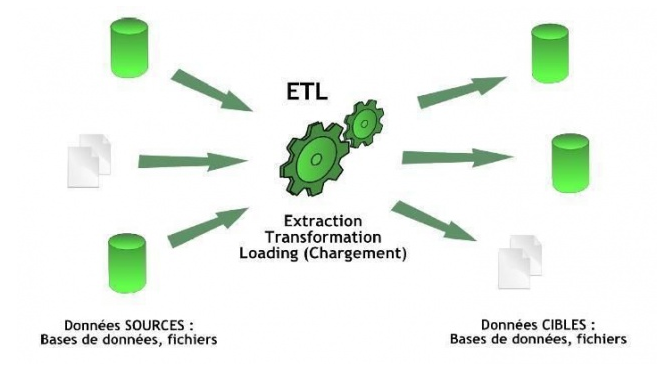
\includegraphics{etl}
    \caption{Extraction - Transformation - Chargement}
    \label{fig:etl}
\end{figure}

\subsection{Notion d’ETL}
L'ETL représente la zone de construction qui contient l’ensemble d’outils et techniques utilisés lors du processus de préparation des données, avant leurs chargements au niveau de l’entrepôt, qui sont utilisés pour alimenter les bases de données opérationnelles qui se situent au niveau du Data warehouse tier. Comme son nom l’indique, l’ETL est un processus à trois étapes.

\subsection{Extraction des données}
Consiste à recueillir des données hétérogènes provenant de multiples sources, base de données opérationnelles, ou des fichiers de différents formats ; ils peuvent être des sources internes à l’organisation ou extérieures. Pour résoudre les problèmes d’interopérabilité, les données sont extraites chaque fois que possible en utilisant l’interface du programme d’application, telles que ODBC (Open DataBase Connection), OLEDB (Open Linking and Embedding for DataBase) et JDBC (Java DataBase Connectivity). \cite{book:10}

\subsection{Transformation des données}
Une fois que les données sont extraites du système source, elles subissent une série de traitements destinée à les transformer en informations présentables.Cette procédure comporte plusieurs aspects : \cite{book:11}
\begin{itemize}
    \item le nettoyage, ce qui supprime les erreurs et les incohérences dans les données et les convertit en un format normalisé ; 
    \item l’intégration, qui concilie les données provenant de différentes sources de données, au niveau schéma et données ; 
    \item et l’agrégation, qui résume les données obtenues à partir de sources de données en fonction du niveau de détail, ou la granularité, de l’entrepôt de données.
\end{itemize}

\subsection{Chargement des données}
Alimente l’entrepôt de données avec les données transformées en respectant les contraintes du SGBD cible. Cela inclut également le rafraîchissement de l’entrepôt de données à savoir, la propagation des mises à jour dans l’entrepôt de données à partir des sources de données à une fréquence spécifiée afin de fournir des données à jour pour le processus de prise de décision. \cite{book:10}

\paragraph{}
Le processus ETL nécessite généralement une zone de préparation de données (data staging). Le data staging représente le chantier de l’ED. C’est là que les données sont chargées, nettoyées, combinées, archivées, puis rapidement exportées vers l’entrepôt. L’objectif de cette zone est l’obtention de données prêtes à être chargées sur un serveur de présentation (un moteur OLAP ou un SGBDR) \cite{book:12}



\section{Les magasins de données ou « datamarts »}
Un Datamart est un sous élément du DataWarehouse , également sous le nom de « magasin de données » ou « comptoir de données » Outil aux prémices du Big Data, son but n’est pas de rassembler des données avant de les trier mais au contraire de les organiser selon des usages métiers ou des domaines ciblés. En effet, sous-ensemble du DataWarehouse, il contient des informations se rapportant à un secteur d'activité particulier de l'entreprise ou à un métier qui y est exercé. Ils servent à des utilisateurs dans l’entreprise et répondent à leurs besoins ; on parle notamment de Datamart financier, de Datamart marketing, de Datamart commercial…
\paragraph{}
Au sein d’une entreprise, les différents services de celle ci auront besoin chacun de données qui leurs seront propres. Le Datamart a justement été crée pour regrouper au sein d’une base ces informations propres à un service ou plus généralement à une fonction. De ce fait, à une fonction correspond un Datamart. Les bases de données pourront être traitées et préparées plus finement, de manière plus orientée et avec une grande précision.
\paragraph{}
Le Datamart rassemble un ensemble de données regroupées, organisées, agrégées et ciblées dans le seul et unique but de répondre aux besoins des métiers. Au sens technique, il est créé à partir d’une base de données relationnelle exploitée à partir du langage informatique SQL\footnote{Structured Query Language, pour les requêtes sur les bases de données} et stockée physiquement sur un disque dur par le biais d’un système de gestion de base de données. Il se situe en aval du DataWarehouse et est alimenté par celui-ci. Les notions que nous venons de decouvrir ainsi que la figure \ref{fig:datamart}, qui démontre la relation entre le Datamart et le Datawarehouse ont étés extraites d'une page web parlant des Datamarts et des Datawarehouse sur le site officiel de SupINFO \cite{WEBSITE:2}
\begin{figure}[H]
    \centering
    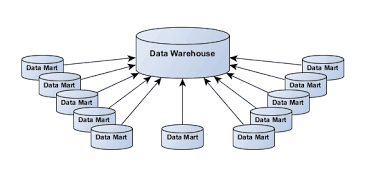
\includegraphics{datamart}
    \caption{Ensemble de Datamarts formant un Datawarehouse}
    \label{fig:datamart}
\end{figure}


\section{Les cubes OLAP}

\subsection{Concept OLAP}
Le terme OLAP (On-Line Analytical Processing) désigne une classe de technologies conçue pour l’accès aux données et pour une analyse instantanée de ces dernières, dans le but de répondre aux besoins de Reporting et d’analyse.
\paragraph{}
R. Kimball définit le concept « OLAP » comme \textit{« Activité globale de requêtage et de
présentation de données textuelles et numériques contenues dans l’entrepôt de données; Style
d’interrogation spécifiquement dimensionnel » }. \cite{book:14}

C’est en continuant sur sa lancée, qui lui a permis de définir le model OLTP pour les bases de données relationnelles, que le concept OLAP fut introduit et défini6 en 1993 par E.F Codd, le père des bases de données relationnelles, dans un document technique portant le titre de « Providing OLAP (On-Line Analytical Processing) to User-Analysts : An IT Mandate ». \cite{ARTICLE:1}

\subsection{Notion de cube}
D'après Mahèzi Magnouwai dans un article \textit{"Cube OLAP, rapports basés sur un cube"} \cite{WEBSITE:6}, un cube OLAP est une base de données à plusieurs dimensions optimisées pour réaliser des applications décisionnelles. Le cube est un outil d’analyse multidimensionnelle destiné aux utilisateurs métier. La figure \ref{fig:olapcube} provient du même article.

\begin{figure}[H]
    \centering
    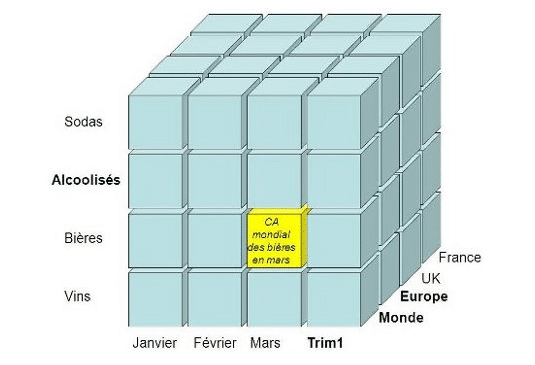
\includegraphics{olapcube}
    \caption{Représentation conceptuel d'un cube OLAP}
    \label{fig:olapcube}
\end{figure}

\paragraph{}
Elle continue en disant que dans les cubes OLAP, les données sont classées par dimension. Les cubes sont pré-synthétisés entre les dimensions et les données sont agrégées afin d’accélérer considérablement l’interrogation par rapport aux bases de données relationnelles. Le cube étant aussi considéré comme une base de données, elle stocke les informations comme le ferait une base de données traditionnelle mais sa structure est différente. Historiquement, les bases de données sont conçues selon les exigences des systèmes informatiques qui les utilisent. En revanche, les cubes OLAP sont exploités par des utilisateurs métiers en vue de faire des analyses. Le cube sert aussi d’une couche entre l’entrepôt de données (datawarehouse) et l’utilisateur final. Un cube OLAP a les caractéristiques suivantes :
\begin{itemize}
    \item il permet d’obtenir des informations déjà agrégées selon les besoins de l’utilisateur. Pas besoin de créer donc un rapport pour chaque besoin de l’utilisateur;
    \item il est simple à utiliser avec des mécanismes de « drag and drop ». Vous n’avez juste qu’à faire des glisser-déposer des données que vous souhaitez analyser. Les cubes sont rapides daccès. Généralement le cube ne contient pas toutes les données de l’entrepôt de données;
    \item il permet d'avoir la possibilité de manipuler des données agrégées selon différentes dimensions (axes);
    \item un cube utilise les fonctions classiques d’agrégation : min, max, count, sum, avg, mais peut également utiliser des fonctions d’agrégations spécifiques.
\end{itemize}
\paragraph{}
Tout comme les bases de données qui ont un langage qui permet de les gerer : le langage est SQL (Structured Query Language) mentionne un peu plus haut, les cubes OLAP disposent également d’un langage appelé le langage MDX (Multidimensional Expression).


\subsection{Langage de navigation : « MDX »}
Le MDX (de l'anglais Multidimensional Expressions, « expressions multidimensionnelles ») est un langage de requête pour les bases de données OLAP, analogue au rôle de SQL pour les bases de données relationnelles. C'est aussi un langage de calcul avec une syntaxe similaire à celle des tableurs.
\paragraph{}
Le langage des expressions multidimensionnelles possède une syntaxe appropriée à l'interrogation et manipulation des données multidimensionnelles mémorisées dans un cube OLAP. Bien qu'il soit possible de traduire certaines expressions dans le langage SQL traditionnel, cela nécessite une syntaxe SQL souvent maladroite même pour des expressions MDX très simples. MDX a été adopté par une large majorité de fournisseur de la technologie OLAP et est devenu un standard de facto pour les systèmes OLAP.


\section{Les systèmes de « reporting »}
Le terme "Reporting" désigne une famille d'outils de Business intelligence destinés à assurer la réalisation, la publication et la diffusion de rapports d'activité selon un format prédéterminé. Ils sont essentiellement destinés à faciliter la communication de résultats chiffrés ou d'un suivi d'avancement.

\subsection{Notion de reporting}
Alain Fernandez dans son article intitulé \textit{"La création et la publication de rapport d'activité"} \cite{WEBSITE:4} nous fait savoir que l'outil de reporting assure l'interrogation des bases de données selon les requêtes SQL préparées lors de l'élaboration du modèle. Le rapport d'activité peut ensuite être publié sur l'Intranet, périodiquement en automatique ou ponctuellement à la demande. L'outil offre bien entendu des fonctions spécifiques pour l'élaboration du modèle du rapport, des modules de calcul et de présentation (graphiques) afin de concevoir des comptes rendus particulièrement seyants et pertinents.
\paragraph{}
Il continue en disant qu'avec les outils requêteurs, l'utilisateur peut formuler des requêtes d'interrogation "ad hoc" à volonté. Les outils de reporting ne sont pas à proprement parlé des instruments d'aide à la décision. Bien que, lorsqu'ils sont utilisés correctement, on peut juger qu'ils permettent au responsable de disposer d'une précieuse vue d'ensemble de son activité, ils sont en fait surtout destinés à "rendre compte" du travail effectué auprès de la hiérarchie. 
\paragraph{}
Le reporting s'inscrit dans une longue tradition du management par le contrôle. Nous sommes bien loin des possibilités d'autonomie que peut offrir la technologie de la Business Intelligence aujourd'hui.

\begin{figure}[H]
    \centering
    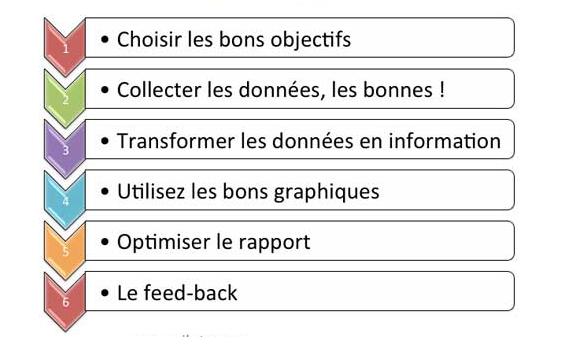
\includegraphics{reportingreussi}
    \caption{Un reporting réussi}
    \label{fig:reportingreussi}
\end{figure}

Provenant du même article, la figure \ref{fig:reportingreussi} montre les étapes à suivre pour obtenir un "rapport réussi". Un "rapport réussi" est un rapport suffisamment pertinent et correctement présenté pour intéresser ses destinataires, soutenir l'attention et susciter des commentaires constructifs.

\subsection{Analyse ad-hoc}
Margaret Rouse dans son article \textit{"Analyse ad hoc"} sur LeMagIT \cite{WEBSITE:5} a ecrit les paragraphes suivants sur l'analyse ad hoc.
\paragraph{}
L'analyse ad hoc est un processus d'informatique décisionnelle (BI) conçu pour répondre à une question métier unique et précise. Le résultat d'une analyse ad hoc est généralement un modèle statistique, un rapport analytique ou une forme quelconque de synthèse des données. 
\paragraph{}
Selon le Larousse, ad hoc « se dit d'une règle, d'un raisonnement élaborés uniquement pour rendre compte du phénomène qu'ils décrivent, ne permettant donc aucune généralisation ». Une analyse ad hoc a pour objet de combler les lacunes laissées par les rapports réguliers, mais statiques de l'entreprise. Elle peut servir à créer un rapport qui n'existe pas encore ou à approfondir un rapport statique pour obtenir des détails sur des comptes, transactions ou enregistrements. Le processus permet également de recueillir des données plus récentes dans les domaines déjà couverts par un rapport statique.
\paragraph{}
Les tableaux de bord OLAP sont spécialement conçus pour faciliter l'analyse ad hoc en offrant un accès rapide et facile aux données du rapport d'origine. En effet, si l'utilisateur (généralement un responsable ou un cadre) peut accéder lui-même aux données par une interface de type « point-and-click », il devient inutile de demander une analyse à une autre entité de l'entreprise. Ainsi, cette fonctionnalité accélère les temps de réponse lorsqu'une question métier se présente, ce qui permet à l'utilisateur de réagir et de prendre ses décisions plus rapidement.
\paragraph{}
Bien que destinés à un usage unique, la plupart des rapports et analyses ad hoc finissent souvent par être réutilisés et exécutés régulièrement. Cette pratique relativement courante peut conduire à des processus superflus, qui se révèlent particulièrement lourds dans les périodes de reporting intense. Par conséquent, il convient de revoir périodiquement les rapports en fonction de critères d'efficacité, afin de déterminer s'ils sont toujours utiles.

\subsection{Reporting de masse}
Tiré du livre blanc de Anne-Marie Abisségué intitulé \textit{"Le reporting de masse : état des lieux et nouveaux enjeux"} \cite{book:13}, le reporting de masse désigne les outils reposant sur des techniques d'interrogation, de reporting et de diffusion automatisées d'une information personnalisée vers un grand nombre d'utilisateurs. L'évolution des systèmes décisionnels en entreprise est poussée par la nécessité de mettre à disposition du plus grand nombre d’employés des outils d’accessibilité à l’information adaptés leurs besoins. L'objectif étant d'avoir une masse d’information pour prendre les bonnes décisions et mettre en place les bonnes actions.
\paragraph{}
A cette étape du développement des systèmes décisionnels, ce sont davantage les capacités de découverte et d'analyse de l'information des outils qui ont été mises en avant. Mais l'utilisation de ces outils présente des contraintes aussi bien en terme de rapidité d'exécution de la requête demandée (plusieurs heures, voire plusieurs jours), qu'en terme de compétence nécessaire pour les manipuler (ces outils mobilisent des analystes spécialisés). Les limites des outils décisionnels traditionnels sont vite atteintes, car leur utilisation reste le fait d'un nombre restreint d'utilisateurs.

\begin{figure}[H]
    \centering
    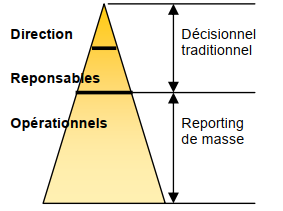
\includegraphics{reportingmasse}
    \caption{La place du reporting de masse}
    \label{fig:reportingmasse}
\end{figure}
 Provenant du même livre que les paragraphes précédentes, la figure \ref{fig:reportingmasse} montre la place du reporting de masse dans l'entreprise. La connaissance et l'analyse de l'information par un petit cercle de personnes dans l'entreprise ne suffisent plus. L'information doit être accessible au plus grand nombre dans l'entreprise, une nécessité imposée par les nouveaux contextes organisationnels.



% \subsection{Les systèmes de visualisation de données}

% \subsubsection{Notion de visualisation des données}
% \blindtext

% \subsubsection{Historique de la visualisation des données}
% \blindtext

% \subsubsection{Fonctions de la visualisation des données}
% \blindtext



\section{Gestion commerciale et décisionnel}
L’entreprise, qu’elle soit multinationale ou une TPE\footnote{Très Petite Entreprise}, doit vendre pour « survivre ». C’est aussi sa vraie mission : la rentabilité ! Pour assurer cette mission, l’aspect commercial est très important. Dans un contexte aussi concurrentiel, l’entreprise ne peut plus se contenter de « vendre » mais doit planifier une vraie stratégie commerciale qui se traduira dans sa gestion commerciale. C’est pourquoi la gestion commerciale est l’un des piliers d’une entreprise qui réussit.
\paragraph{}
La gestion commerciale s’occupe de toute la chaîne nécessaire à la production de biens/services en vue de leur vente. Elle va donc prendre en charge la prévision, la réalisation et le suivi des ventes. La gestion commerciale englobe aussi bien la fonction achat, que la logistique ou encore la facturation et la vente (dont celle de l’après-vente). 

\subsection{Importance de la gestion commerciale}
Marion, en 2017 \cite{WEBSITE:3} dans son article \textit{"L’importance de la gestion commerciale en entreprise"} dit que pour trouver la bonne solution gestion commerciale, il convient d’en comprendre la notion. Cette procédure englobe tous les besoins liés à la production des biens ou services pour la vente. Cette gestion prend ainsi en charge de la prévision, de la réalisation et du suivi des ventes. Elle réunit également la fonction d’achat, la logistique ou encore la facturation et l’après-vente. À titre de rappel, une bonne gestion commerciale assure le pilotage de l’entreprise. C’est la gestion commerciale qui s’occupe de fixer les prix de vente des services ou des produits, effectuer le suivi des stocks ou encore la gestion des relations clients ainsi que la gestion des relations avec les fournisseurs. On entend par là les relances des créances impayées. C’est également en se basant sur les données du département commercial que les dirigeants pourront prendre des décisions stratégiques. 

\subsection{Objectifs des outils de gestion commerciale}
Facturation, suivi de livraison, relances client… La gestion commerciale est un service clé de l’entreprise. Elle est facilitée par des outils de gestion informatique de plus en plus efficaces.

L'objectif principal de la gestion commerciale est de réaliser, prévoir et développer la vente des biens ou des services. Les fonctions commerciales sont présentes aussi bien dans le B to B (business to business, qui désigne la vente aux entreprises) que dans le B to C (business to consumer, qui signifie « vente au grand public »).

Elle est prévue pour optimiser la chaîne de valeur des entreprises (ensemble d'activités interdépendantes visant à générer de la valeur) en regroupant les processus internes.

La gestion commerciale s’occupe de toute la chaîne nécessaire à la production de biens et services. Ses missions principales sont :
\begin{itemize}
    \item la conquête de nouveaux clients ;
    \item le développement de clients et de projets ;
    \item le développement d’activités à l’international ;
    \item le développement de partenariats stratégiques, afin de préparer la croissance future.
\end{itemize}
La gestion commerciale fournit également les indicateurs de marché permettant aux dirigeants de réaliser les choix stratégiques pertinents.

\subsection{Fonctions des outils de gestion commerciale}
Selon l’Association pour l'Emploi des Cadres (APEC)\footnote{https://recherche-d-emploi.ooreka.fr/comprendre/apec}, la gestion commerciale recrute plus de 30 000 cadres par an. En pratique, cette filière s’articule autour des fonctions suivantes :
\begin{itemize}
    \item achat et relations avec les fournisseurs ;
    \item fixation des prix de vente ;
    \item prévision, réalisation, relations, suivi des stocks ;
    \item vente, facturation, fidélisation et relances clients ;
    \item contrôle de gestion commerciale.
\end{itemize}
\paragraph{}
Dans le détail, les logiciels de gestion commerciale, de dernière génération permettent :
\begin{itemize}
    \item la création de devis, factures et bons de livraison ;
    \item la gestion des comptes et commandes client ;
    \item le suivi des achats et des ventes ;
    \item le transfert des données en comptabilité ;
    \item l’édition des les relevés des clients en attente de paiement ou de facturation (balance âgée) ;la gestion des stocks en temps réels ;
    \item la gestion des commerciaux.
\end{itemize}




 



\section*{Conclusion}%
\addcontentsline{toc}{section}{\numberline{}Conclusion}%
%Le but de ce chapitre étant de faire une revue de littérature, sortir la problématique, étudier l’existant et proposer une solution, nous en ressortons que l’entreprise a besoin d’une plateforme de Business Intelligence pour pallier a ses problèmes de fixation des prix et comment savoir quels produits seront demandés pour des périodes spécifiques.
Le but de ce chapitre étant de faire une revue de littérature pour présenter les concepts qui seront abordés dans ce projet, nous avons fait le tour des notions et concepts et nous sommes à présent armés de connaissances qui nous seront utiles pour la suite du projet.
